\section{DevOps}

De acordo com \cite{zalla} quando uma empresa precisa entregar uma nova versão do software ao usuário, é necessário por parte da equipe de desenvolvimento e de operações uma comunicação mais efetiva para que essa demanda não atrase o andamento do projeto. Por exemplo, surge com frequência a necessidade de instalação e configuração de requisitos do sistema operacional para que os programas e serviços funcionem corretamente. Isso se transforma em uma tarefa de configuração complexa e custosa, principalmente se a empresa possui alto número de servidores, computadores e elevados padrões de governança. Para resolver esse problema surge o conceito de DevOps \cite{zalla}.

De acordo com \cite{amazon} o DevOps é a combinação de filosofias, práticas e ferramentas que aumentam a capacidade de distribuir aplicativos e serviços em alta velocidade. Essas velocidade permite que seus clientes sejam atendidos de forma melhor e as empresas conseguem competir de forma mais eficaz no mercado.

DevOps é complementar ao desenvolvimento ágil, inserindo-se no processo de integração contínua e entrega contínua utilizando ferramentas como Docker ou Vagrant, assegurando que o código está pronto para produção além de permitir um melhor fluxo de trabalho entre as duas equipes \cite{medrado}.

Com esse novo modelo, as equipes de desenvolvimento e operações não são mais separadas, ou seja, os engenheiros trabalham durante todo o ciclo de vida do aplicativo, da fase de desenvolvimento e testes à fase de implantação e operações.

\begin{figure}[H]
	\centering
  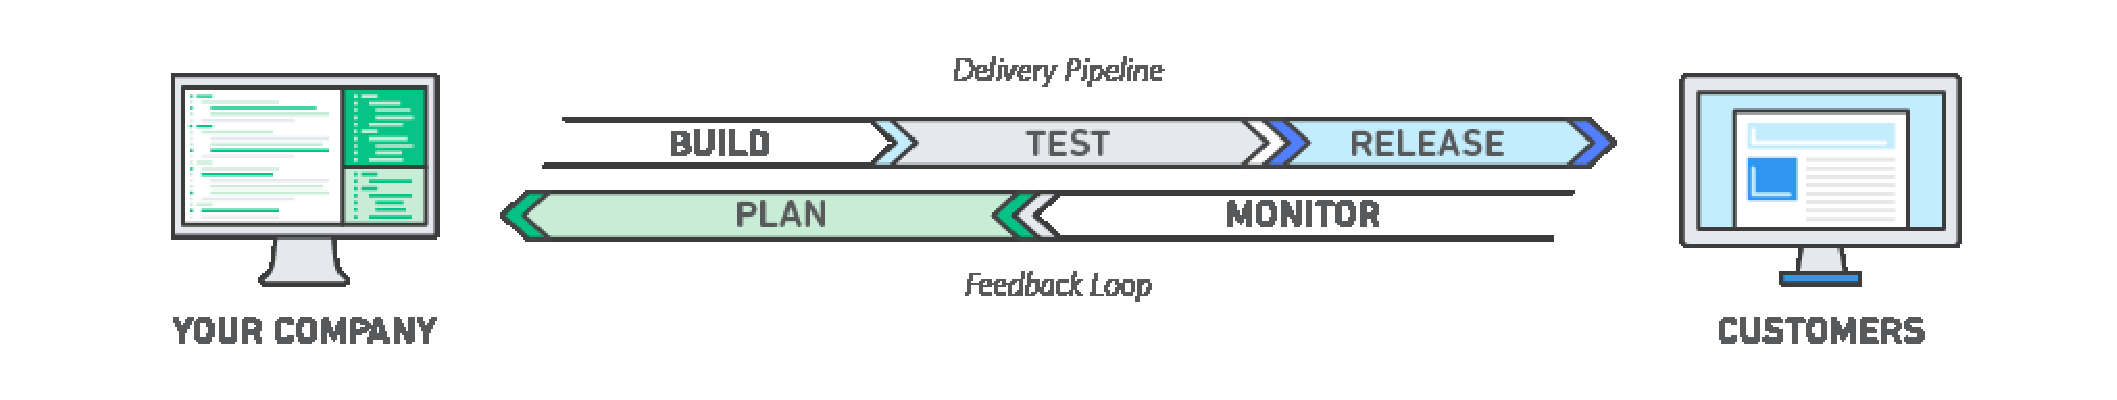
\includegraphics[keepaspectratio=true,scale=0.4]{figuras/devops_pipe.eps}
  \caption[O que é DevOps.]{O que é DevOps. Fonte: \cite{amazon}}
	\label{fig:devops2}
\end{figure}

\subsection{Benefícios do DevOps}

De acordo com \cite{amazon} os benefícios do DevOps são:

\begin{itemize}
  \item \textbf{Velocidade}: O modelo de DevOps permite que as equipes de desenvolvimento e operações operem em alta velocidade para que se possa trazer inovações para os seus clientes rapidamente, adaptando-se ao mercado.
  \item \textbf{Entrega rápida}: Aumenta o ritmo de lançamento de novas versões com maior frequência e qualidade por meio da integração e entrega contínuas.
  \item \textbf{Confiabilidade}: Garante a qualidade dos lançamentos para que você possa entregar com confiança em um ritmo mais rápido.
  \item \textbf{Escala}: Utilizando infraestrutura como código ajuda a gerenciar sistemas complexos ou dinâmicos com eficiência e risco reduzido.
  \item \textbf{Colaboração melhorada}: As equipes de desenvolvimento e operações colaboram de perto, compartilham responsabilidade e combinam seus fluxos de trabalho.
  \item \textbf{Segurança}: Mantem o controle e preserva a conformidade.
\end{itemize}

\subsection{Fechamento da seção}

O DevOps proporciona uma mudança cultural que tem como foco as práticas de automação das diversas atividades necessárias para agilizar e entregar código de qualidade em produção e estão frequentemente ligadas ao desenvolvimento ágil. Por exemplo: compilação do código, testes automatizados, empacotamento, criação de ambientes para testes e produção, configuração da infraestrutura do software, migração de dados, monitoramento, melhoria de logs e métricas, segurança, desempenho e deploy \cite{sato} citado por \cite{correa}.
